\makeatletter\let\ifGm@compatii\relax\makeatother
\documentclass[aspectratio=169]{beamer}
\usepackage[norules,nolineno]{lgrind}
\usepackage{changepage}
\usepackage{hyperref}
\usetheme{Berlin}
\usecolortheme{dolphin}
\title{Hearthstone Card Replacer}
\author{Jordan Carey, Brian Lascuna, Muhammed Mahmood, Cameron Mellott}
\institute{Ohlone College CS102}
\date{8 November 2016}
\hypersetup{colorlinks=true, linkcolor=blue}

\begin{document}
\beamertemplatenavigationsymbolsempty

\begin{frame}{Specification}
The purpose of this program is to find replacement Hearthstone cards. 
This is done by taking the card name the user inputs and entering it into
the Hearthstone API (\url{market.mashape.com/omgvamp/hearthstone}) to find the 
attributes (e.g. mana cost, attack, health, 
class) of the card. The program then stores these attributes and finds 
replacements by comparing them with cards of the same 
type. If too few cards are found, the program broadens the scope of the search.
After the search is complete, the program displays the images of the 3 best 
replacements cards.
\end{frame}

\begin{frame}[allowframebreaks]{Analysis}
\begin{center}
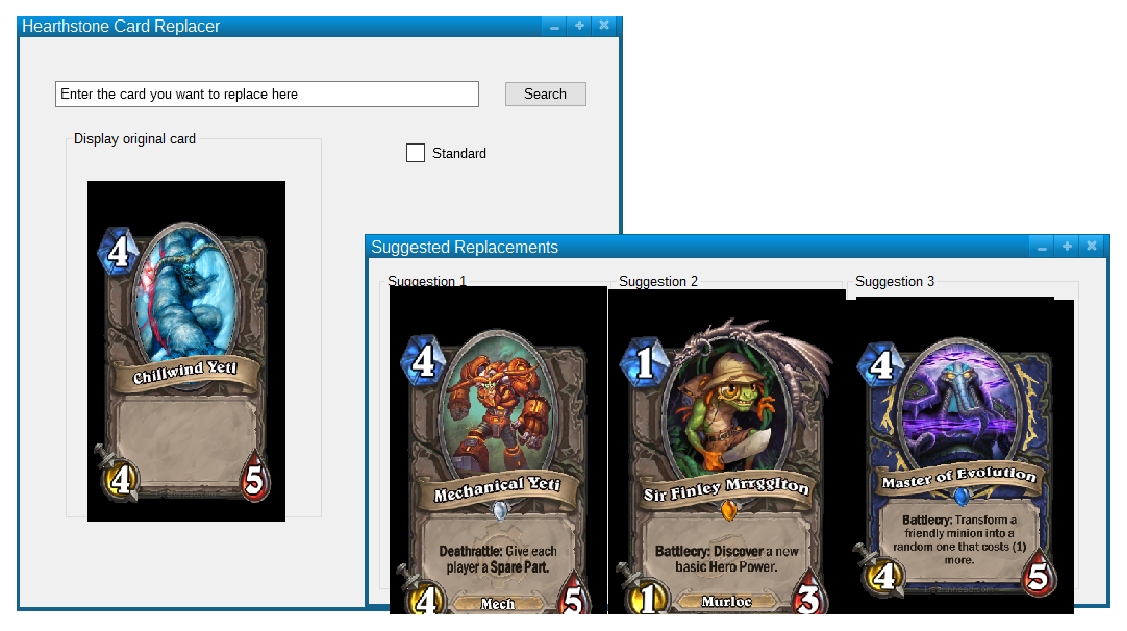
\includegraphics[width=3in]{Analysis.eps}
\end{center}
This is a mock up of our GUI design. The user will input the name of a card and
press the button to call our event handler which will look up the input card,
run our comparison algorithm, and return a new window frame showing the three
best matches.\\
\pagebreak
To look up the cards, we will use OMGVAMP's Hearthstone API hosted at
\url{market.mashape.com/omgvamp/hearthstone}. We will use the CURL library to 
retrieve card data from the API and write it into a file, then use
Niels Lohmann's JSON library to parse the file
into data structures we can use in our comparisons. The GUI will be made using
FLTK's Cairo library.
\\

\end{frame}

\begin{frame}[allowframebreaks]{Design}
\begin{itemize}
\item compareMinions
\begin{itemize}
\item If user's card is a minion, retrieve a list of legal minions
\item Iterate through the list comparing each card to the user's to determine fitness
\item If the cost of both cards is equal, the fit is increased by 3
\item Otherwise, fit is reduced by 3 times the difference
\item If the health of both cards is equal, the fit is increased by 3
\item Otherwise, fit is reduced by 2 times the difference
\item If the attack of both cards is equal, the fit is increased by 3
\item Otherwise, fit is reduced by 3 times the difference
\end{itemize}

\pagebreak
\item compareSpell
\begin{itemize}
\item If user's card is a spell, retrieve a list of legal spells
\item Iterate through the list, comparing each card's text to determine fitness
\item Tokenize the text of the card into individual words and compare the words
to the user's card's text
\item If a word in the card's text matches one in the user's, fit is increased by 3
\item If a matching word is a mechanic keyword, fit is increased by an additional 5
\item Fit is reduced by the square of the difference in cost
\end{itemize}

\pagebreak
\item compareWeapons
\begin{itemize}
\item If user's card is a minion, retrieve a list of legal minions
\item Iterate through the list comparing each card to the user's to determine fitness
\item If the cost of both cards is equal, the fit is increased by 3
\item Or if the user's card costs more, fit is reduced by the difference squared
\item Or if the user's card costs less, 
fit is reduced by 2 times the square of the difference
\item If the durability of the user's weapon is lower, the fit is increased by 2
times the difference
\item Otherwise, fit is reduced by 3 times the difference
\item If the attack of user's card is lower, the fit is increased by the difference
\item Otherwise, fit is reduced by 2 times the difference
\end{itemize}

\end{itemize}
\end{frame}

\begin{frame}[allowframebreaks]{Implementation}

Main\\
Goal: Start the GUI and pass control to FLTK
\lgrindfile{main}
\pagebreak

getCard\\
Goal: Retrieve data for a single card from the Hearthstone API
\begin{itemize}
\item Access API using Mashape key
\item Use JSON library to parse data
\item Store card data in a struct
\end{itemize}
\lgrindfile{getCard}
\pagebreak

getData\\
Goal: Retrieve a set of card data to compare against the search card
\begin{itemize}
\item Access the Hearthstone API's type endpoint for the type matching the 
search card
\item Use snippets from CURL documentation to write retrieved data into a file
\item Use JSON library to parse file into a list of card structs
\end{itemize}
\lgrindfile{getData}
\pagebreak

compareMinions\\
Goal: Assign scores to possible replacement minions
\begin{itemize}
\item Iterate through the list of minions provided by getData
\item Compare the cost, health, and attack of the search card to each minion in
the list
\item Return a list of legal replacements with similarity scores calculated
\end{itemize}
\lgrindfile{compareMinions}
\pagebreak

compareSpell\\
Goal: Assign scores to possible replacement spells
\begin{itemize}
\item Iterate through the list of spells provided by getData
\item Turn the text value of the card into tokens
\item Compare the text of each spell in the list to the search card by matching
tokens
\item Return a list of legal replacements with similarity scores calculated
\end{itemize}
\lgrindfile{compareSpell}
\pagebreak

compareWeapons\\
Goal: Assign scores to possible replacement weapons
\begin{itemize}
\item Iterate through the list of weapons provided by getData
\item Compare the cost, durability, and attack of the search card to each weapon
in the list
\item Return a list of legal replacements with similarity scores calculated
\end{itemize}
\lgrindfile{compareWeapons}
\pagebreak

cullCards \\
Goal: Find the three most similar cards to the search card
\begin{itemize}
\item Iterate through the list of cards provided by the compare functions
\item Compare the similarity scores against each other, keeping the three highest
\item Return a list of the three cards with the highest similarity score
\end{itemize}
\lgrindfile{cullCards}
\pagebreak

GUIWindow \\
Goal: Create a GUI for the user to enter a search query to find replacement cards
\begin{itemize}
\item Create a Cairo window using FLTK
\item Create a user input field and a field to hold the image
\item Send user input to cbSearch function when user presses button
\end{itemize}
\lgrindfile{GUIWindow}
\pagebreak

makeDisplayWindow \\
Goal: Create a window to display the top three replacement cards
\begin{itemize}
\item Create a Cairo window using FLTK
\item Create three boxes to hold card images
\item Call compare function matching type of user's card
\item Call cullCards to cull comparisons to three best fits
\item Retrieve card images from list returned by cullCards and display in order
of fit
\end{itemize}
\lgrindfile{makeDisplayWindow}
\pagebreak

cbSearch \\
Goal: Call getCard to find data on card entered by user and display its image
\begin{itemize}
\item Send user input to getCard
\item Use CURL to download card image
\item Display image in search window
\item Call makeDisplayWindow
\end{itemize}
\lgrindfile{cbSearch}

\end{frame}

\begin{frame}[allowframebreaks]{Test}
The results of a search for the minion card Chillwind Yeti.
\\

\includegraphics[height=1.8in]{yeti}
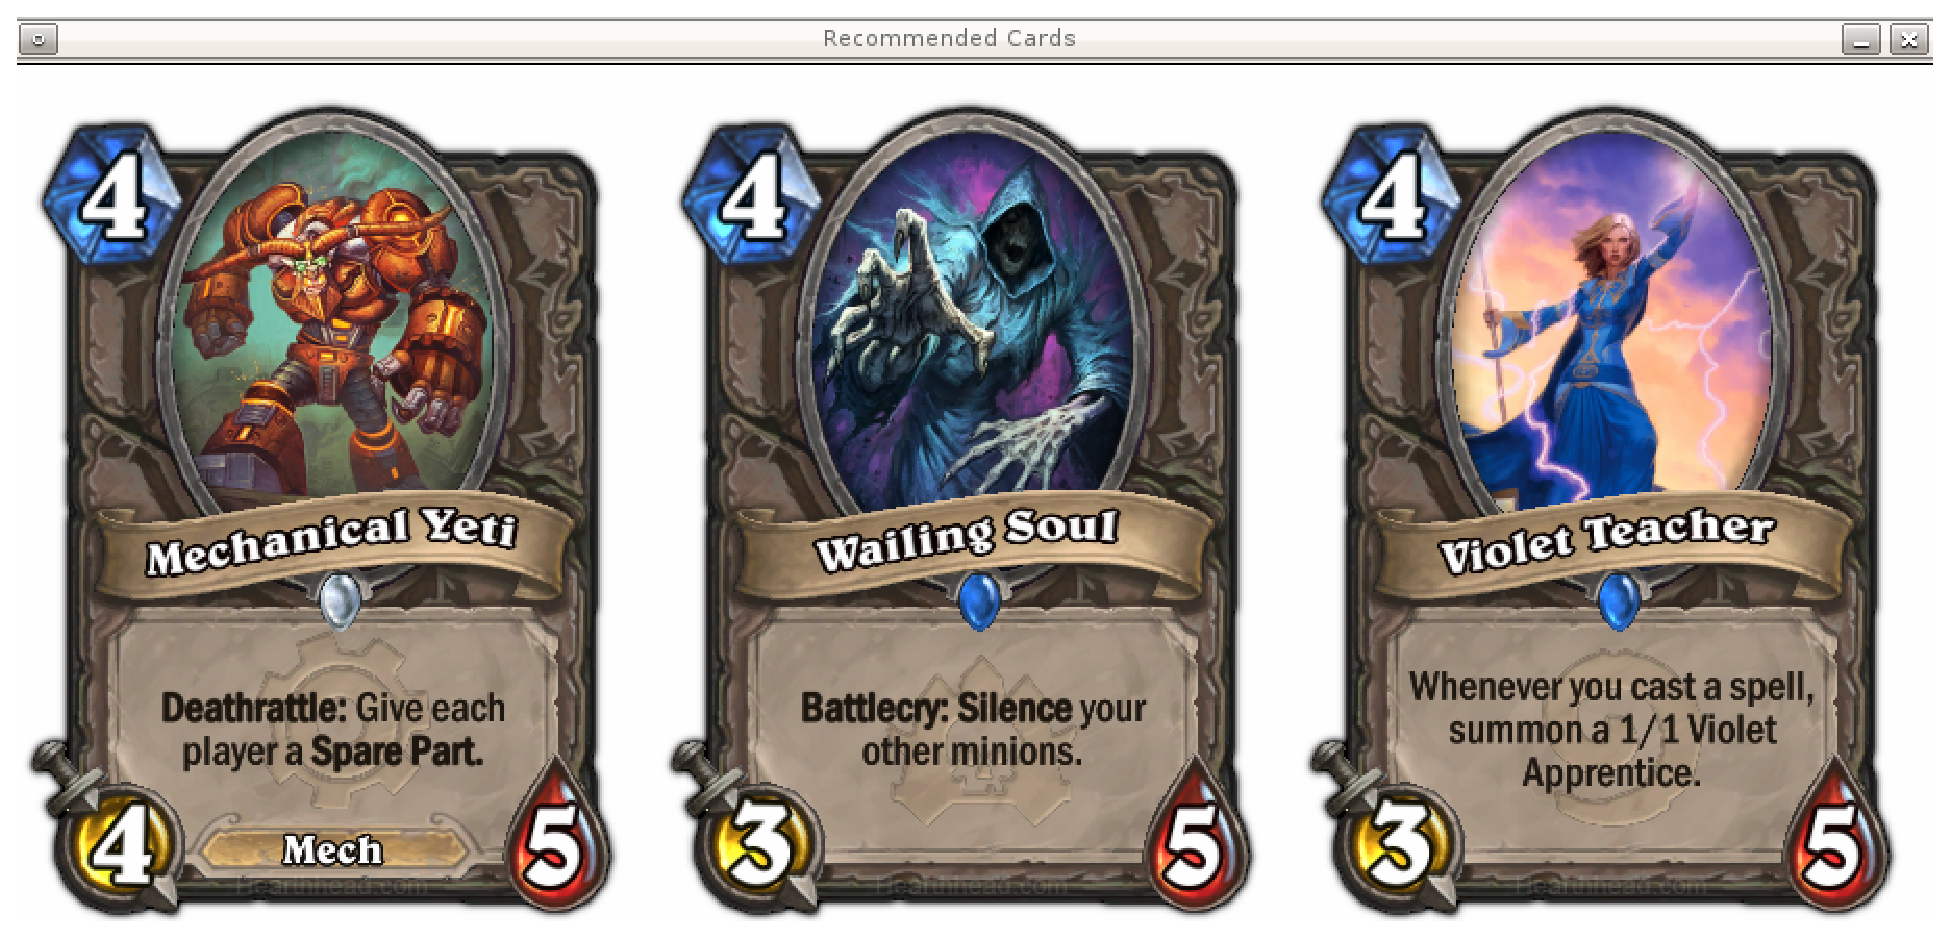
\includegraphics[height=1.6in]{yetiresults}

\pagebreak

The results of a search for the spell card Frost Nova.
\\

\includegraphics[height=1.8in]{nova}
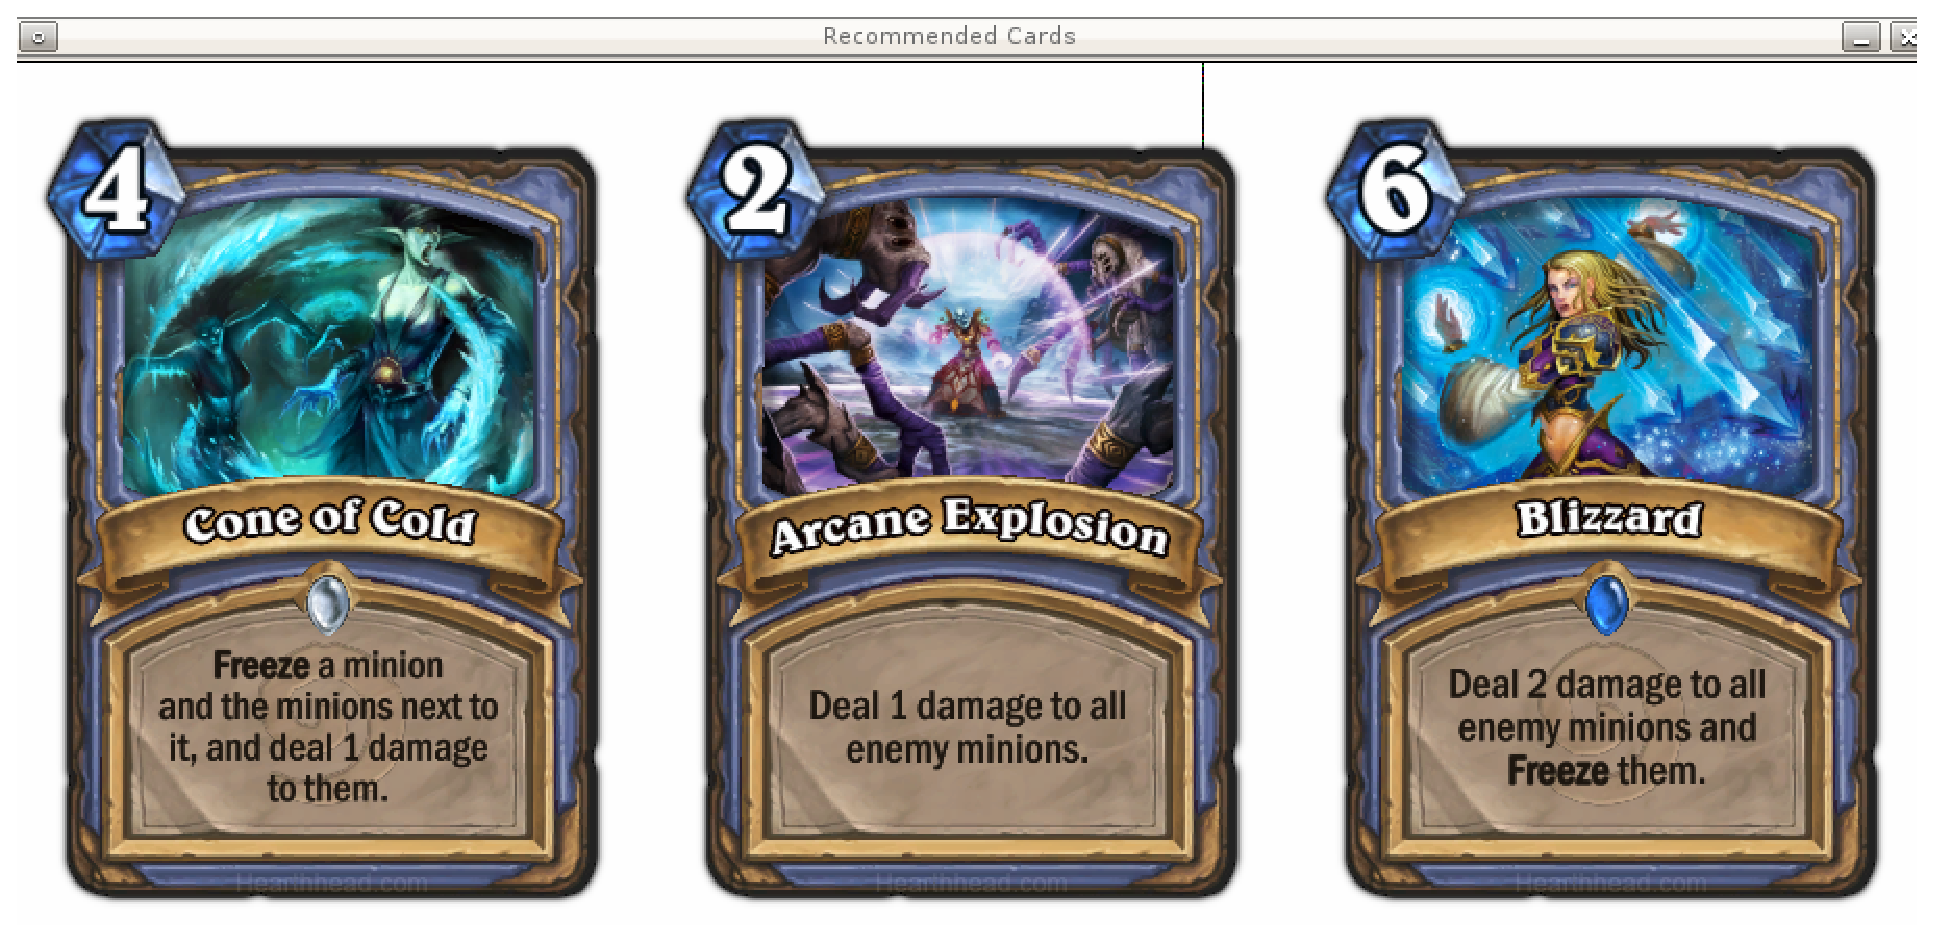
\includegraphics[height=1.6in]{novaresults}

\pagebreak

The results of a search for the weapon card Arcanite Reaper.
\\
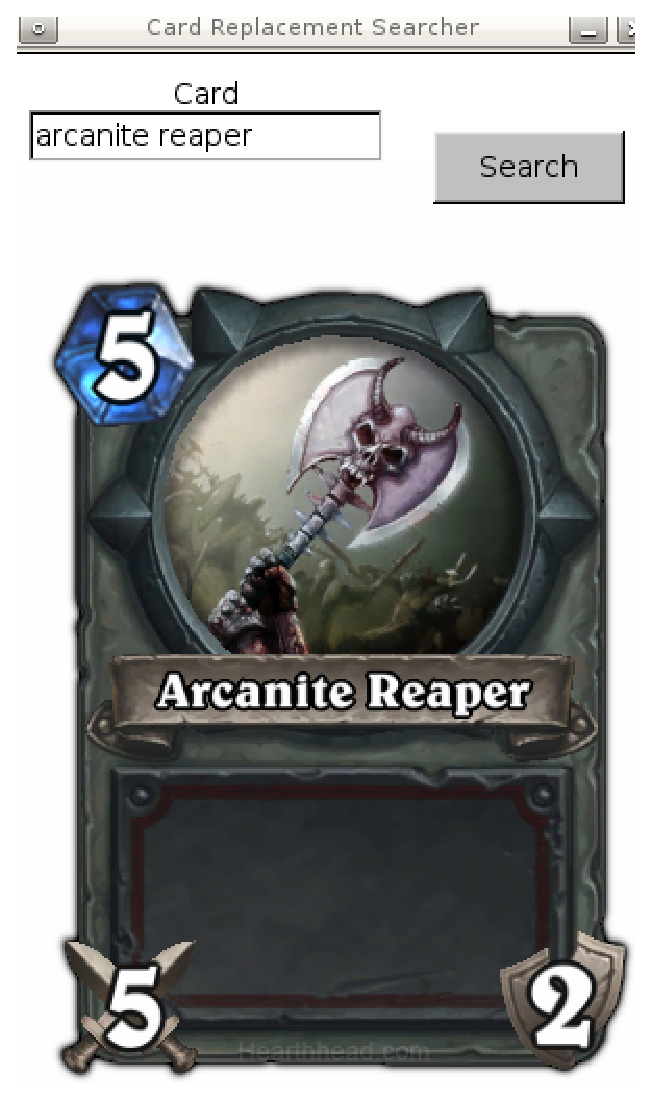
\includegraphics[height=1.8in]{arcanite}
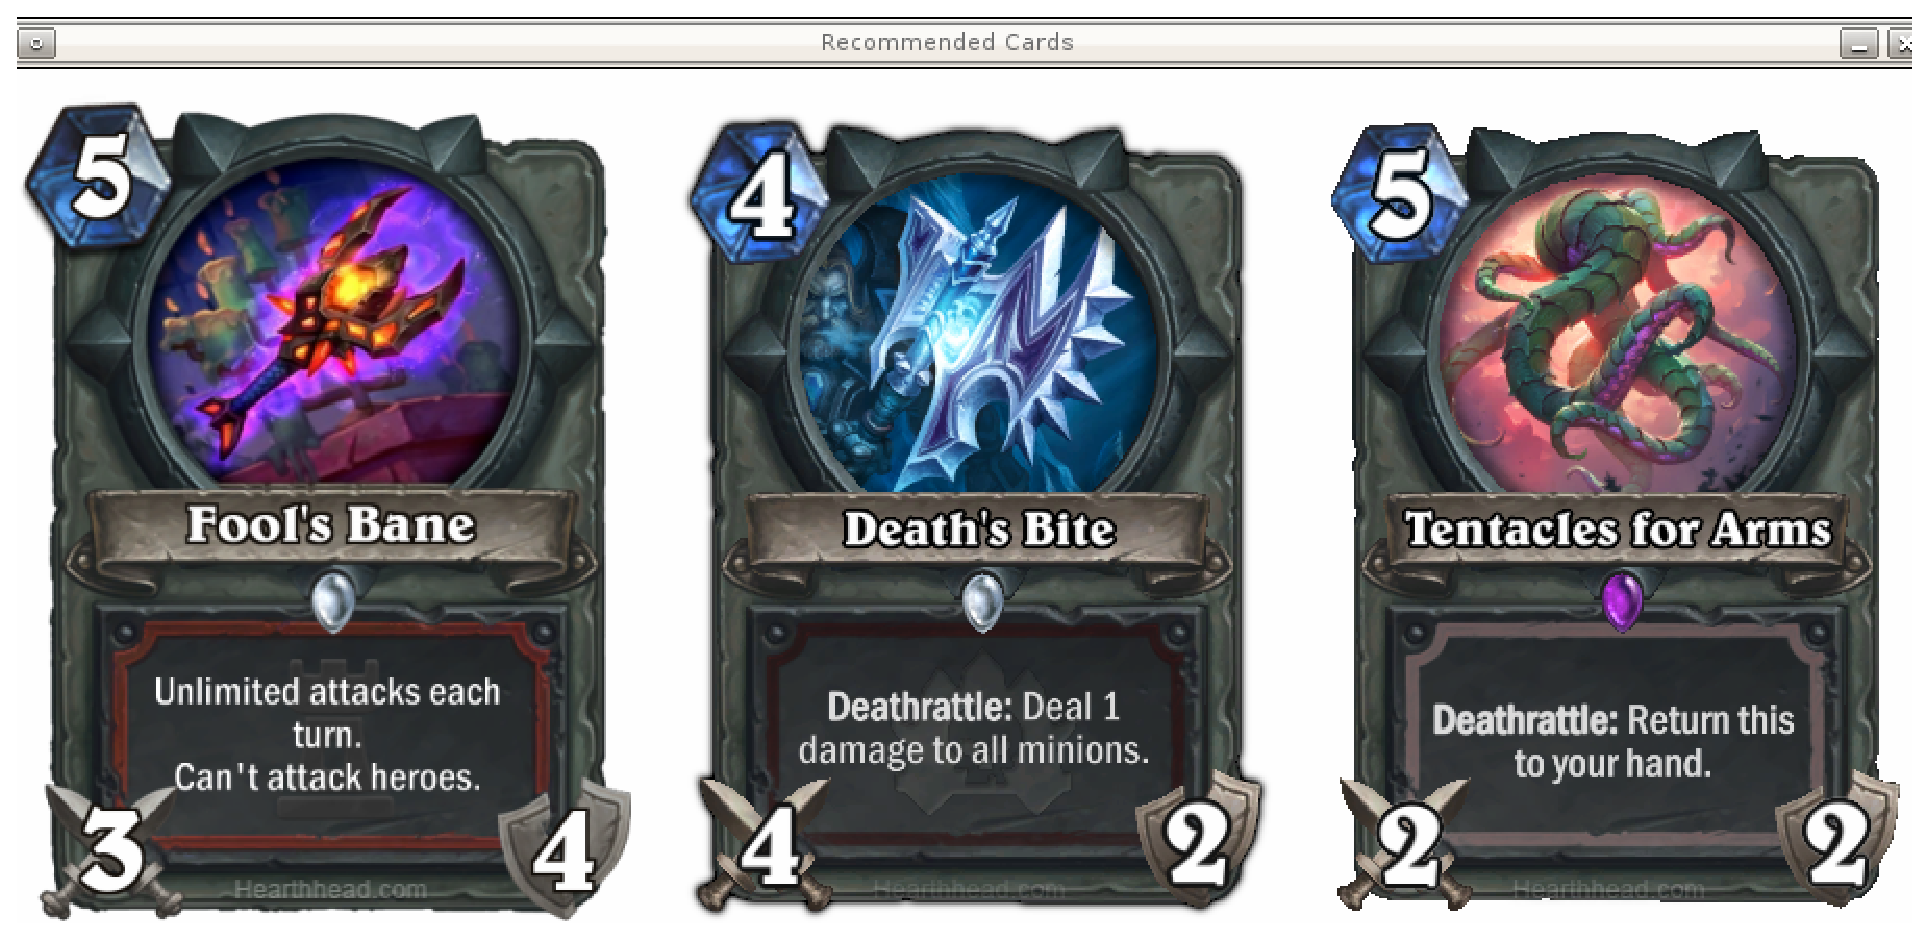
\includegraphics[height=1.6in]{arcaniteresults}

\end{frame}

\end{document}
